\documentclass{article}

\usepackage{fullpage}
\usepackage[colorlinks=true]{hyperref}
\usepackage[tableposition=top]{caption}
\usepackage[utf8]{inputenc}

\usepackage{Sweave}
\begin{document}
\Sconcordance{concordance:Body_weight_figure_EJS.tex:Body_weight_figure_EJS.Rnw:%
1 7 1 1 0 8 1 1 17 2 1 1 27 3 1 1 15 1 2 3 1 1 2 1 1 1 2 10 0 1 2}


\title{Analysis of Body composition of C57BL6/J mice exposed in utero to MCP230 and saline}
\author{Erin Stephenson}
\date{\toWeek}
\maketitle

\section*{Data}
This script uses the \verb+Sheet1+ from \verb+Bodyweight_analysis_week.xlsx+ and is located in the \verb+C:/Users/esteph16/Documents/GitHub/ObesityParticulateTreatment/scripts/Bodyweight_analysis_week_EJS+ directory.  This analysis was most recently run on Thu Dec 03 12:24:23 2015.  

\section*{Data Summary}
\Section*{Figures}

\begin{figure}
\begin{center}
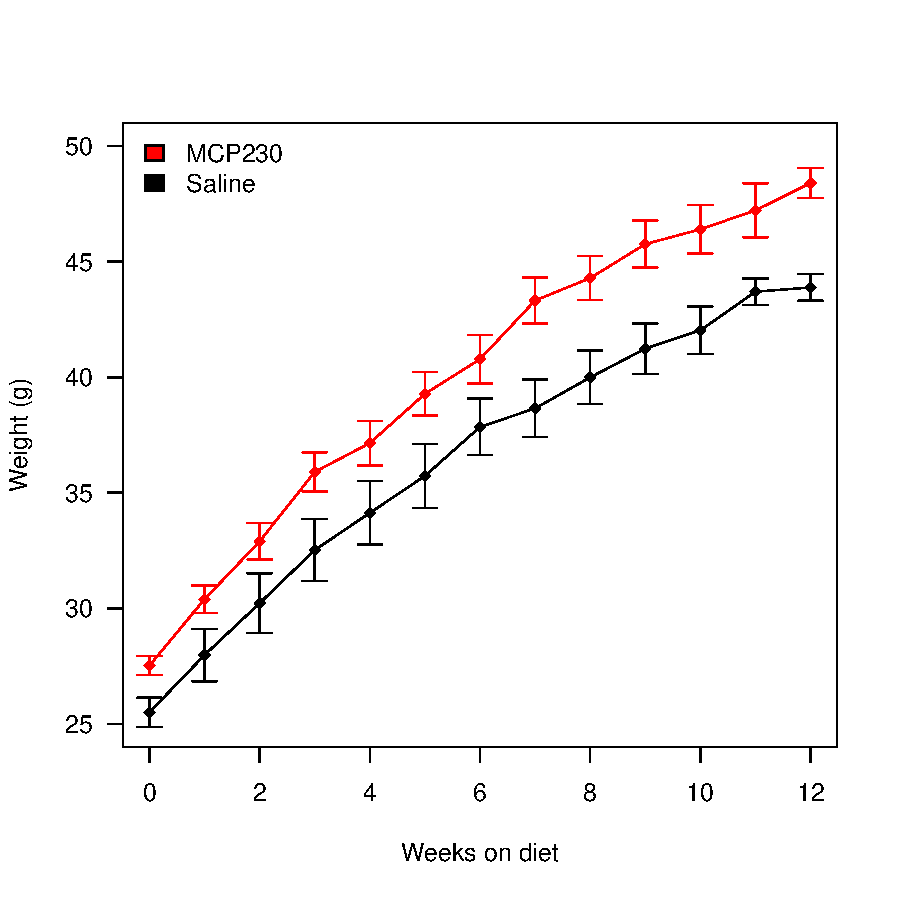
\includegraphics{Body_weight_figure_EJS-lineplotWeight}
\end{center}
\caption{Lineplot of fed weights}
\label{fig:lineplotweight}
\end{figure}

\section*{Session Information}
\begin{itemize}\raggedright
  \item R version 3.1.1 (2014-07-10), \verb|x86_64-w64-mingw32|
  \item Locale: \verb|LC_COLLATE=English_United States.1252|, \verb|LC_CTYPE=English_United States.1252|, \verb|LC_MONETARY=English_United States.1252|, \verb|LC_NUMERIC=C|, \verb|LC_TIME=English_United States.1252|
  \item Base packages: base, datasets, graphics, grDevices, methods,
    stats, utils
  \item Other packages: dplyr~0.4.1, lme4~1.1-10, Matrix~1.2-3,
    plyr~1.8.3, rJava~0.9-7, xlsx~0.5.7, xlsxjars~0.6.1
  \item Loaded via a namespace (and not attached): assertthat~0.1,
    DBI~0.3.1, grid~3.1.1, lattice~0.20-29, lazyeval~0.1.10,
    magrittr~1.5, MASS~7.3-33, minqa~1.2.4, nlme~3.1-117, nloptr~1.0.4,
    parallel~3.1.1, Rcpp~0.12.2, splines~3.1.1, tools~3.1.1
\end{itemize}\end{document}
